%%%%%%%%%%%%%%%%%%%%%%%%%%%%%%%%%%%%%%%%%%%%%%
\section{Run Plan}
\label{sec:runplan}

\fixme{Need to update the run plan when Nikos's H4 simulation results are available}

At present the H4 beamline simulation results are not available. To estimate the beam rates, we use inputs from a generic target simulation based on 100k 80 GeV $\pi^+$ beam on 15 cm copper target. This $\pi^+$ rate is roughly equivalent to 10\% of a typical SPS spill. The distributions of the tertiary particles from the copper target are shown in Figure~\ref{fig:beamline_target}. The figure on the left is for postively charged and the figure on the right is for negatively charged tertiary particles. 
\begin{cdrfigure}[Target simulation]{beamline_target}{Simulated flux of charged secondary particles resulting from 100k $\pi^+$ each with an energy of 80~GeV impinging on a 15 cm copper target. The figure on the left is for positively charged and the figure on the right is for negatively charged secondary particles.}
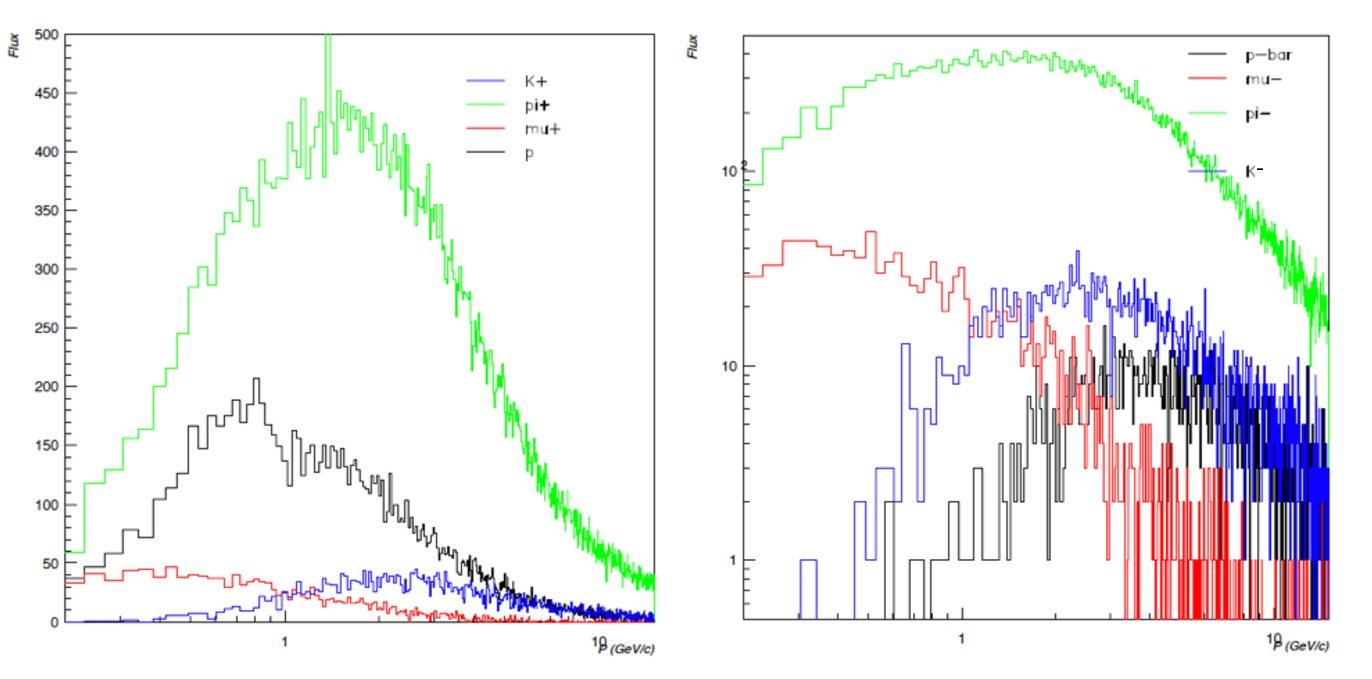
\includegraphics[width=0.8\textwidth]{beamline_CuTarget.jpg}
\end{cdrfigure}

To formulate a preliminary beam time request, we assume the hadron beam rates and spectrum as given in Figure~\ref{fig:beamline_target}. For the beam rate estimates, we account for particle decays assuming the distance from the secondary target to the cryostat to be 30 m. A significant fraction of pions and kaons below 1 GeV/c decay before reaching the liquid argon cryostat. In addition, we also assume the data taking efficiency to be about 50\%. For the electron sample, we expect a different optimized beamline setup to produce a pure electron beam with a flux of about 200 Hz. A preliminary run plan for one configuration is shown in Table~\ref{tab:RunPlan}. 
%
\begin{table}[p]
\centering
\rowcolors{0}{gray!30}{gray!30}
\begin{tabular}{|c|c|c|c|c|c|c|}
\hline
\multicolumn{7}{|c|}{\bf Positive Sample} \\ \hline
\bf $P$ & \bf $\#$ of Spills & \bf Time & \bf $\#$ of $\pi^+$ & \bf$\#$ of $\mu^+$ & \bf$\#$ of $K^+$ & \bf$\#$ of p \\ 
\bf (GeV)& & \bf (hours) & & & & \\ \hline
\hiderowcolors
0.2&900 &11&\textcolor{red}{\bf 15k} &180k&$\approx$0&160k\\ 
0.3&200 &3 &\textcolor{red}{\bf 15k} &30k &$\approx$0&50k \\
0.4&150 &\textcolor{red}{\bf 2} &22k &18k &$\approx$0&32k \\ 
0.5&150 &\textcolor{red}{\bf 2} &26k &12k &$\approx$0&38k \\
0.7&150 &\textcolor{red}{\bf 2} &40k &10k &$\approx$0&45k \\
1  &350 &4 &120k&\textcolor{red}{\bf 10k} &$\approx$0&65k \\
2  &600 &8 &320k&\textcolor{red}{\bf 10k} &3k        &130k\\
3  &500 &6 &290k &\textcolor{red}{\bf 5k} &7k        &70k \\
5  &1800&23& 1M &\textcolor{red}{\bf 5k}  &5k        &270k\\
7  &1200&15&660k&\textcolor{red}{\bf 6k}  &3k        &120k\\ \hline
Total &6000&76&2.5M  & 286k  &18k   & 1M\\
\hline \hline
\multicolumn{7}{|c|}{\bf Negative Sample} \\ \hline
\showrowcolors 
\bf $P$ & \bf $\#$ of Spills & \bf Time & 
\multicolumn{2}{|>{\columncolor[gray]{0.83}}c|}{\bf $\#$ of $\pi^-$ }& 
\multicolumn{2}{|>{\columncolor[gray]{0.83}}c|}{\bf$\#$ of $\mu^-$ } \\ 
\bf (GeV)& & \bf (hours) & 
\multicolumn{2}{|>{\columncolor[gray]{0.83}}c|}{}& 
\multicolumn{2}{|>{\columncolor[gray]{0.83}}c|}{} \\ \hline  
\hiderowcolors
0.2&600&8&\multicolumn{2}{|c|}{\textcolor{red}{\bf 15k}} &\multicolumn{2}{|c|}{88k}\\
0.3&200&3&\multicolumn{2}{|c|}{\textcolor{red}{\bf 15k}} &\multicolumn{2}{|c|}{30k}\\
0.4&150&\textcolor{red}{\bf 2}&\multicolumn{2}{|c|}{30k} &\multicolumn{2}{|c|}{18k}\\
0.5&150&\textcolor{red}{\bf 2}&\multicolumn{2}{|c|}{40k} &\multicolumn{2}{|c|}{13k}\\
0.7&150&\textcolor{red}{\bf 2}&\multicolumn{2}{|c|}{50k} &\multicolumn{2}{|c|}{12k}\\
1  &150&\textcolor{red}{\bf 2}&\multicolumn{2}{|c|}{70k} &\multicolumn{2}{|c|}{12k}\\
2  &200&3&\multicolumn{2}{|c|}{135k}&\multicolumn{2}{|c|}{\textcolor{red}{\bf 6k}}\\ \hline
Total  &1600&22&\multicolumn{2}{|c|}{350k}&\multicolumn{2}{|c|}{180k}\\ 
\hline 
\hline
\multicolumn{7}{|c|}{\bf Electron Sample} \\ \hline
\showrowcolors 
\multicolumn{3}{|>{\columncolor[gray]{0.83}}c|}{\bf $P$} &\bf $\#$ of Spills&\multicolumn{2}{|>{\columncolor[gray]{0.83}}c|}{\bf Time}&{\bf $\#$ of electron }\\
\multicolumn{3}{|>{\columncolor[gray]{0.83}}c|}{\bf (GeV)} & &\multicolumn{2}{|>{\columncolor[gray]{0.83}}c|}{\bf (hours)}&\\
\hline
\hiderowcolors
\multicolumn{3}{|c|}{0.2,0.3,0.4,0.5,0.7,1,2,3,5,7}  & 150 per bin & \multicolumn{2}{|c|}{2 hours per bin} &{140k per bin} \\ \hline
\multicolumn{3}{|c|}{Total}  & 1500 & \multicolumn{2}{|c|}{20} &{1.4M} \\ \hline
\end{tabular}
\caption{A preliminary run plan for one beam angle and position. The number of spills needed for a given momentum bin is driven by the samples highlighted in red or by the requirement of at least 150 spills per momentum bin.}
\label{tab:RunPlan}
\end{table}
The number of spills needed for each momentum bin is driven by the samples highlighted in red. The minimum beam time requirement is 150 spills ($\approx$ 2 hours of beam time) per momentum bin to ensure we have sufficient data taken with stable beam running.  This proposed plan satisfies the requested samples from the physics groups, except for kaons less than 1 GeV. \fixme{Need the physics sample requirement table from the Measurement group}. Most low momentum kaons produced from the secondary target decay before reaching the liquid argon cryostat. To obtain those samples, we will need to carry out extended runs and trigger exclusively on particles tagged as kaons by either the time-of-flight or the threshold Cherenkov counters.

In addition to the above samples with beam at the nominal position, we expect to take some additional data with the beam entering the TPC at different position and angles. Without a detail beamline simulation, there are still some uncertainties on the actual beam rates.  Based on the current information available, the total estimated beam time needed to carry out the physics program in this proposal is in the range of 4 to 6 weeks.
 



